\section{The Sterile Neutrino Hypothesis}\label{sec:sterileResults}
With the null ($3\nu$) hypothesis normalized to the IceCube Monte Carlo as in Eq.~\ref{eq:MC_norm}, we are now in good shape to study the sterile neutrino effect on the probabilities, and how that compares to data
\footnote{We do not consider DeepCore nor PINGU in the sterile neutrino analysis because the $\Pamam$ resonance does not appear in the \si{\GeV} region for \si{\eV^2}-scale $\dm[41]$, as shown in Fig.~\ref{fig:sterile_resonance}.
We bring DeepCore and PINGU back in the next section.}.
First, let us see how the collected data from Fig.~\ref{fig:IC_data} deviates from the predicted $3\nu$ oscillations.
\begin{figure}
    \centering
    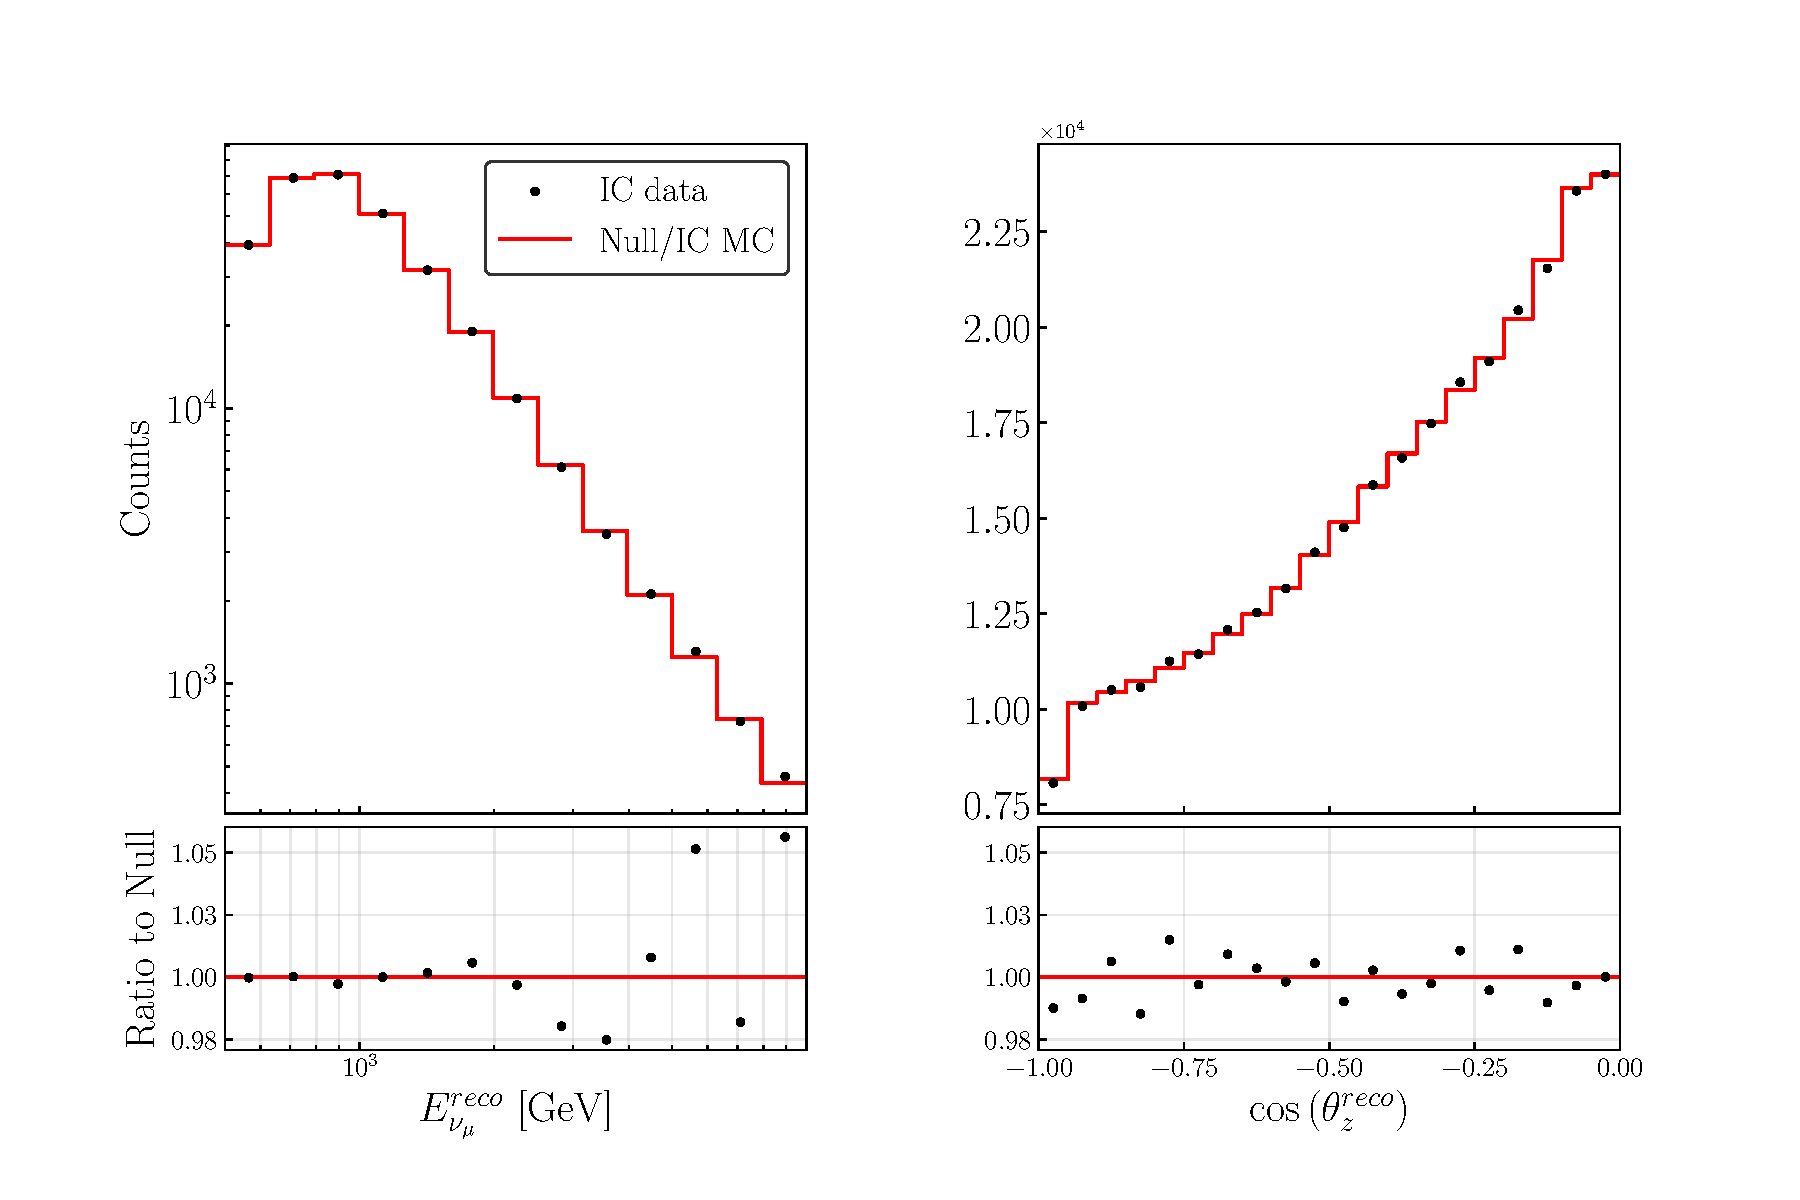
\includegraphics[width=1\textwidth]{figures/IC_rates.pdf}
    \caption{How the IceCube null hypothesis from~\cite{IC2020} compares to their collected data.}\label{fig:IC_rates}
\end{figure}
Fig.~\ref{fig:IC_rates} shows an impressive agreement to the standard $3\nu$ oscillation picture, with the largest deviations of $~6\%$
for neutrinos at $\SI{10}{\TeV}$ values. In zenith, the data only deviates $\pm 2\%$.


\subsection{\texorpdfstring{$\chi^2$}{Chi-squared} Minimization}
For our analyses, we define our $\chi^2$ as
\begin{align} \label{eq:chisq}
    \chi^{2}(\hat{\theta},\alpha,\beta)=\sum_{ij} \frac{\left(N^\text{th}-N^\text{data}\right)_{ij}^{2}}
    {\left(\sigma^\text{data}_{ij}\right)^{2} + \left(\sigma^\text{syst}_{ij}\right)^{2}}+ 
    \frac{(1-\alpha)^2}{\sigma_\alpha^2} + \frac{\beta^2}{\sigma_\beta^2}\,
\end{align}
where we minimize over the model parameters $\hat{\theta}$, the penalty terms $\alpha$ and $\beta$.
$N_{ij}^\text{th}$ is the expected number of events from theory, and $N_{ij}^\text{data}$ is the observed number of events in that bin. 
We set $\sigma_\alpha = 0.25$ as the atmospheric flux normalization error, and $\sigma_\beta = 0.05$ as the zenith angle slope error~\cite{hondapaper}. 
The observed event number has an associated Poissonian uncertainty $\sigma_{ij}^\text{data} = \sqrt{N_{ij}^\text{data}}$.
For IceCube, the event count takes the form
\begin{align}
    N^\text{th}_{ij} = \alpha\left[1+\beta (0.5 + \zreco_i )\right] N_{ij}(\hat{\theta})\,,
\end{align}
with $N_{ij}(\hat{\theta})$ from Eq.~\ref{eq:MC_norm}. Here, the term $ \beta (0.5 + \zreco_i )$ allows the event distribution to rotate with angle $\beta$ around the median zenith angle of $\zreco = -0.5$.
We also have an uncorrelated systematic error $\sigma_{ijk}^\text{syst}$. We set $\sigma_{ijk}^\text{syst} = f\sqrt{N_{ijk}^\text{data}}$, where $f$ is a factor of our own choosing.

The minimization of Eq.~\ref{eq:chisq} simply returns a value for each set of model parameters. We use this value to quantify to what extent
our theoretical simulations $N^\text{th}_{ij}$ agree with the data $N^\text{data}_{ij}$ within the error bounds provided by $\sigma_a,\sigma_b,$ and $f$.
We then select the smallest set of $\chi^2$ values, and our allowed parameters are then their associated $\hat{\theta}$.
We then translate the $\chi^2$ distribution by subtracting the best-fit point, and analyze $\Delta \chi^2 = \chi^2 - \chi^2_{min}$.
From the $\chi^2$-distribution, one can show that the $90\%$ confidence level has a value of $2.71$ for two degrees of freedom. When slicing through the 
two-dimensional grid of $\Delta \chi^2$ at this level, we then obtain a contour plot that tells us what parameter values are within our $90 \%$ confidence level and what regions are not.

\subsection{Sterile Mass and Mixing}
Let us start with looking at the best-fit event distribution resulting from the $\chi^2$ minimization.
Fig.~\ref{fig:final_rate_plot} now contains the best-fit event distribution assuming the 3+1 hypothesis.
The best-fit values are $\dm[41] = \SI{0.01}{\eV\squared}$ and 
$\sin(2\theta_{24})^2 = 0.67$ ($\theta_{24} = \SI{27.5}{\degree}$). 
The contour plot shown in Fig.~\ref{fig:error_tuning} divides the parameter space into two regions.
To the right of the boundary, the $\Delta \chi^2$ has values above the confidence level, meaning that 
those parameter pairs can be excluded at a certain confidence level.

By tuning the scaling $f$ of the uncorrelated systematic error, we can shift the contour. We extract the contour from the 
IceCube sterile neutrino analysis~\cite{IC2020}, and compare in Fig.~\ref{fig:error_tuning}. We see that the contour in the 
higher $\dm[41]$ region above \SI{1}{\eV\squared} is very sensitive to the tuning, while the lower region between \SIrange[]{1e-1}{1}{\eV\squared}
remains fixed. Using the case of 15\% uncorrelated systematic error, we obtain best-fit values of $\dm[41] = \SI{0.01}{\eV^2}$ and $\theta_{24} = 0.67$ ($\sin^22\theta_{24} = 0.95$) at 
a p-value of $20\%$. This is not statistically significant, 
hence we find no evidence for a sterile neutrino within the parameter range $0.01 \le \dm[41] \le \SI{1}{\eV^2}, 0.01\le \sin(2\theta_{24})^2 \le 1$  in IceCube data.
\begin{figure}
    \centering
    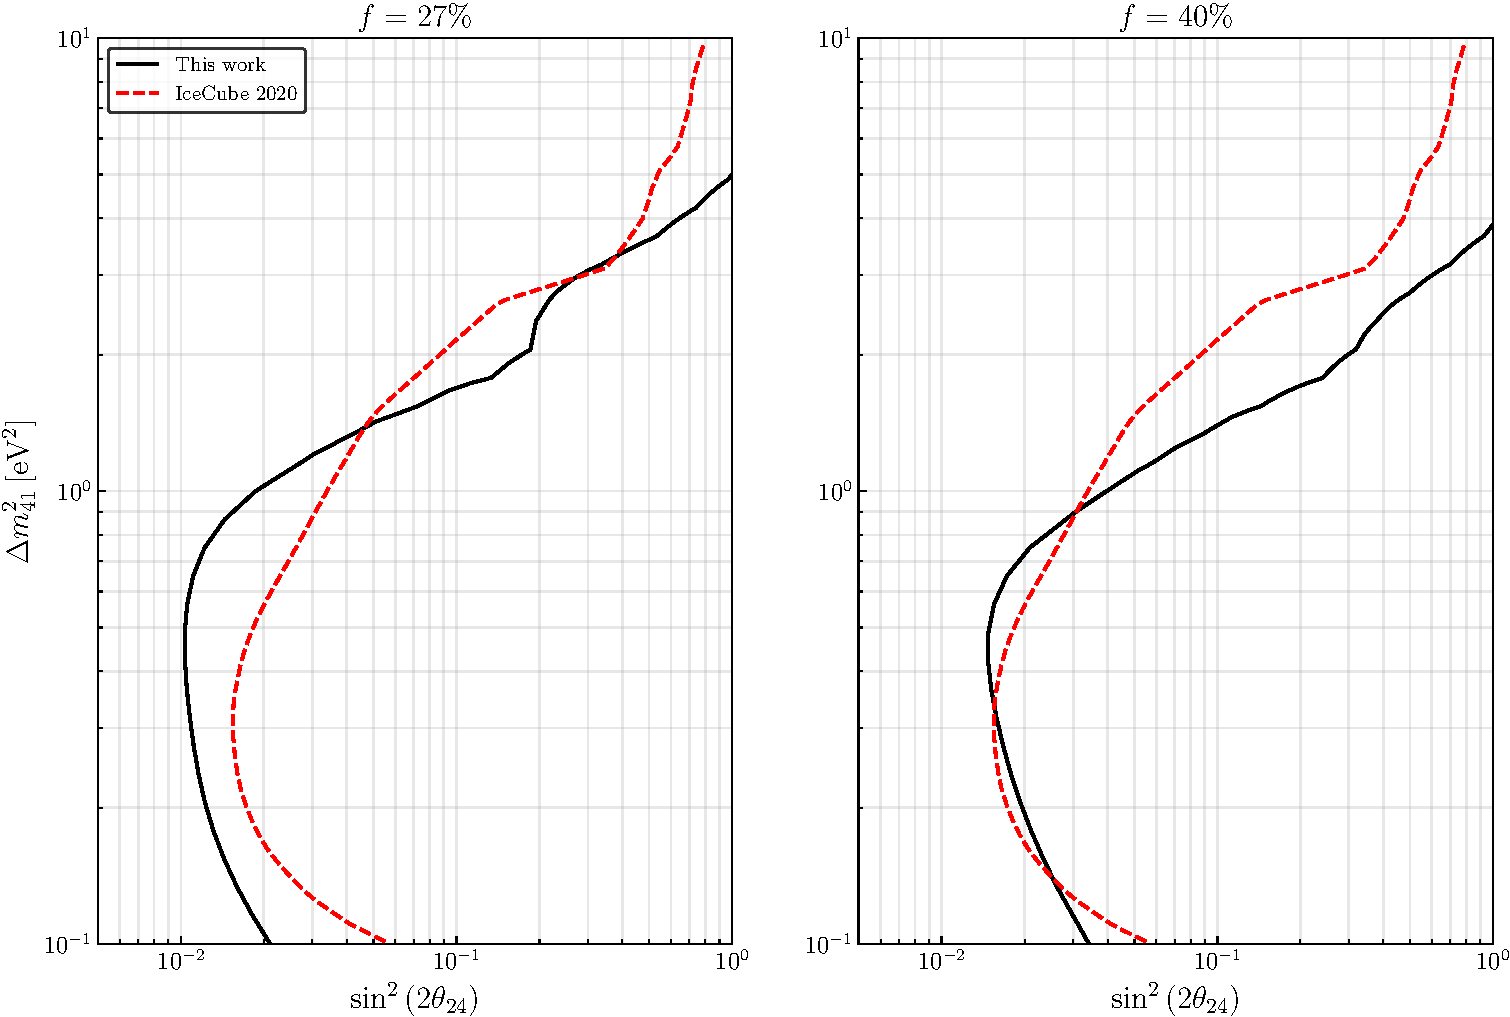
\includegraphics[scale=0.58]{figures/s24_error_tuning.pdf}
    \caption{The 90\% CL contour with two different systematic error scalings, compared 
    with the official IceCube result from~\cite{IC2020}.}\label{fig:error_tuning}
\end{figure}

We now in Fig.~\ref{fig:final_rate_plot} plot the best-fit 3+1 hypothesis with the data from Fig.~\ref{fig:IC_rates}, to finally see how the best 
3+1 hypothesis compares to data.
\begin{figure}
    \centering
    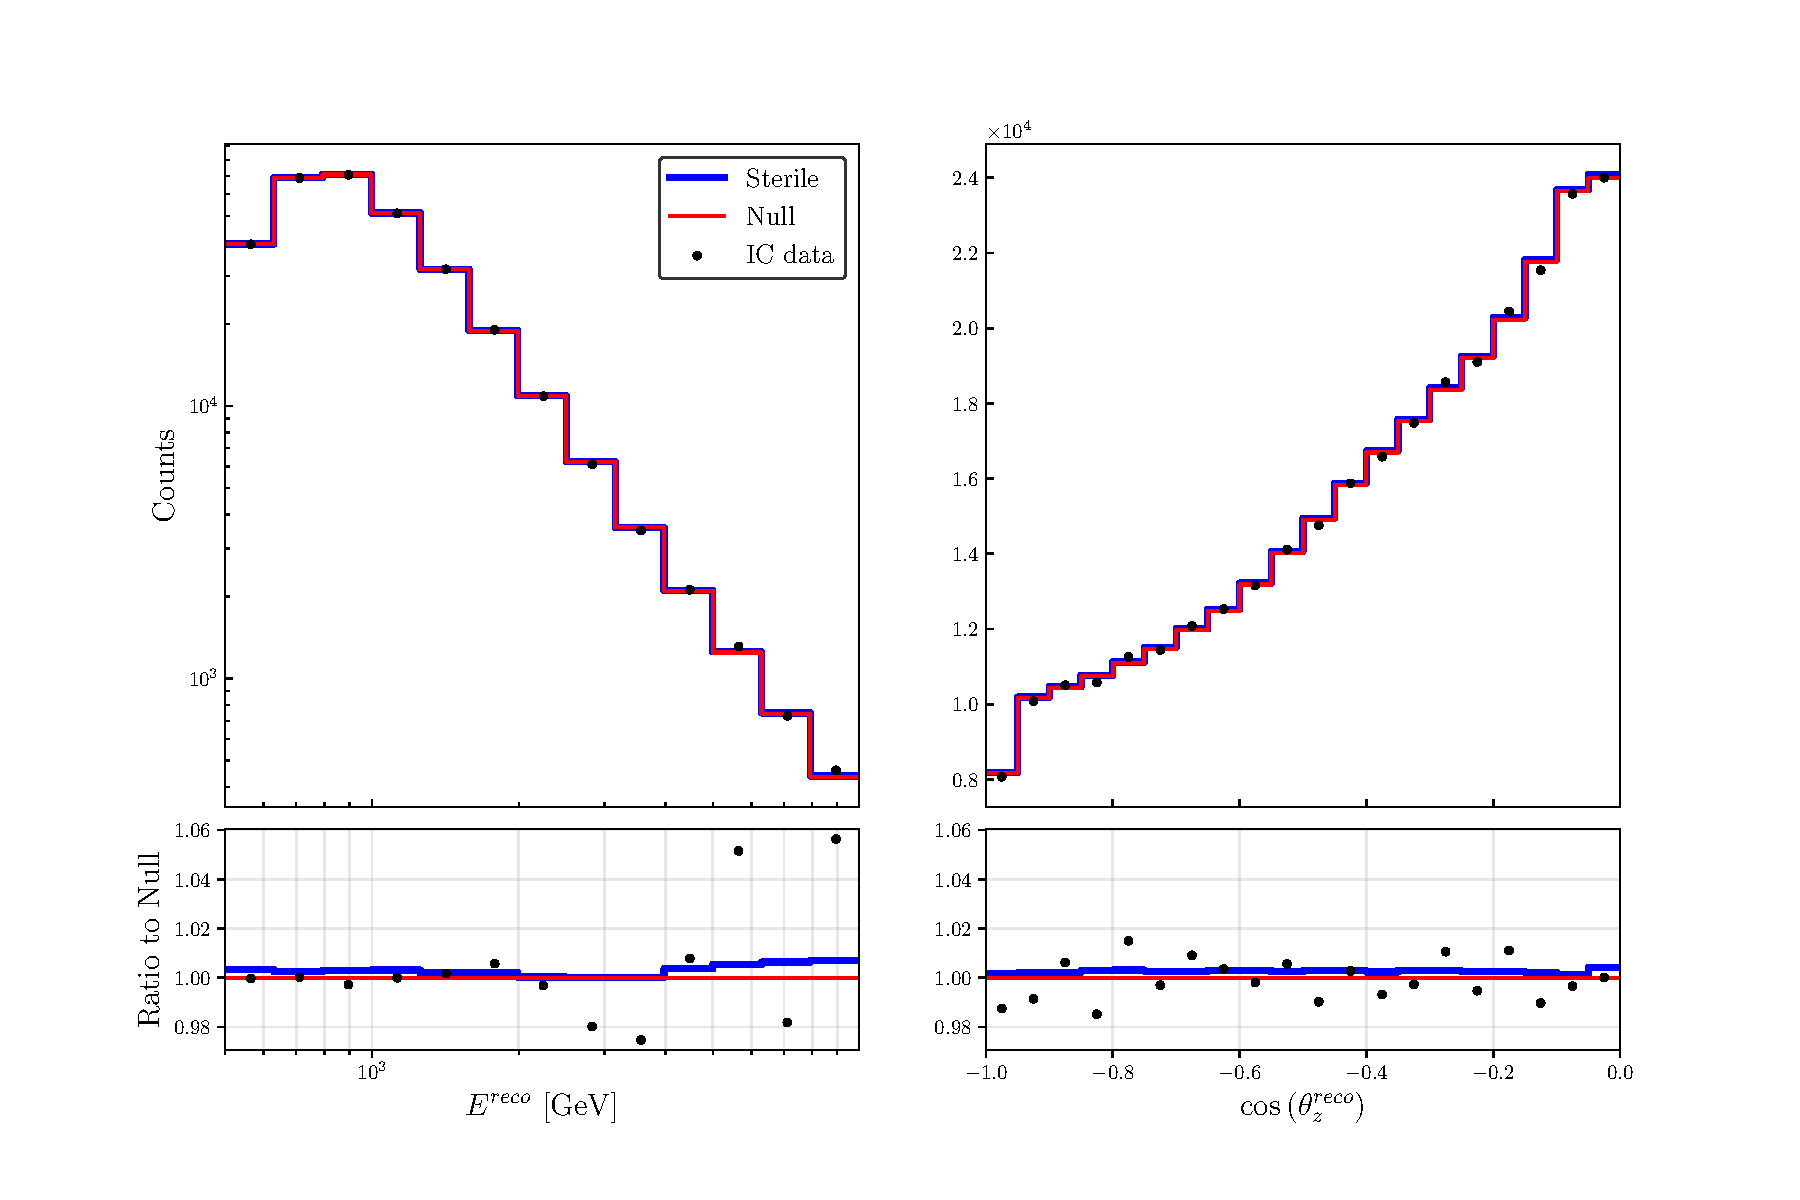
\includegraphics[width=1\textwidth]{figures/final_rate_plot.pdf}
    \caption{The predicted binned event count assuming our best-fit 3+1 hypothesis in blue with $\dm[41] = \SI{0.01}{\eV^2}$ and $\theta_{24} = 0.67$, compared with the 
    null 3+0 hypothesis in red and data points from ~\cite{IC2020} in black.}\label{fig:final_rate_plot}
\end{figure}

Wanting to investigate the effect of $\theta_{34}$, we also simulated the 3+1 hypothesis using $\theta_{24} = \theta_{34}$. However, we did not see 
a difference in the exclusion regions compared to the regions when $\theta_{34} = 0$. Thus, we conclude that in our work, IceCube was not able to 
distinguish any effect due to the $\theta_{34}$ parameter. However, since our dataset only included muon track events in the \SIrange{0.5}{10}{\TeV} range,
one might be able to expect a larger effect of $\theta_{34}$ if one includes cascade events as well.